\chapter{Functional Description} \label{functional-description}

The AHB-Lite Memory IP is a flexible, fully configurable, IP that enables designers to attach internal device memory to AHB-Lite based host. The width and depth of the memory, together with an optional registered output stage, are specified via parameters.

\begin{figure}[th]
	\centering
	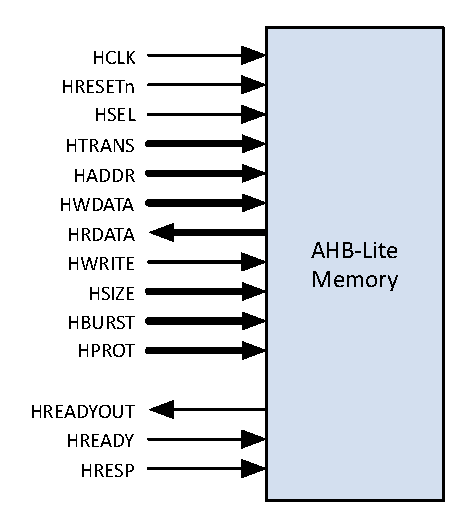
\includegraphics{assets/img/AHB-Lite-Memory-PortDiag}
	\caption{AHB-Lite Memory Signalling}
	\label{fig:ahb-lite-memory-portdiag}
\end{figure}

The IP is designed to easily support a wide range of target
technologies, automatically implementing technology-specific memory
cells according to the chosen target. A generic behavioural
implementation is also supported.

\section{AHB-Lite Bus Locking Support} \label{ahb-lite-bus-locking-support}

The \emph{AMBA 3 AHB-Lite v1.0} protocol supports bus locking. Typically a locked transfer is used to ensure that a slave does not perform other operations between the read and write phases of a transaction. Given the AHB-Lite Memory IP performs no such operations, bus locking is not supported and does not provide the \texttt{HMASTLOCK} input associated with this capability